\chapter{基于点云生成对抗网络的三维重建}
\label{cha:exp}
\section{动机}
在第 \ref{section:pointsetgen} 节中,我们详细地讨论了基于图片的三维点云重建算法 PointSetGen \cite{pointsetgen},% 工作
%的主要内容,
并指出了其两点不足:
\begin{itemize}
	\item 需要用户提供 mask 信息:用户体验差;
	\item 泛化能力差:对于训练数据集中未曾出现的新图像,PointSetGen 有可能失败。
\end{itemize}
本文工作的核心目标正是针对以上两点不足进行改进。

我们将在此章中详细地讲解与分析本工作的
%相关
算法流程与模型架构。
为了便于描述,我们首先定义本工作试图解决的问题。

\section{问题描述 \label{section:myquestion}}
在本工作中,用户需要提供的仅仅是一张三维物体的 RGB 图像 $\bm I$。%,且不含 mask 信息。
我们的目标之一是改善用户体验。因此,不像 PointSetGen,我们不再需要用户提供 mask 信息。

随后,算法需要根据用户提供的输入图像,以点云
$S = \{(x_i, y_i, z_i)^T\}_{i=0}^{N - 1}$
的形式重建出三维模型的完整结构,包括遮挡与不可见的部分。
为了简化问题,我们假设重建结果中点云的点数 $N$ 为固定常数 $N = \numprint{2048}$。
此处的 $N$ 是 PointSetGen 中的两倍,因为我们希望向用户呈现一个更稠密、更完整的重建结果。

此外,我们希望提升算法对于新数据的泛化能力,即相比于 PointSetGen,重建输出的质量应当得到增强。

更进一步的,我们还希望提升用户对于重建系统的可控制性。
具体而言,我们希望用户可以按照其期望,
对于多个已有的重建结果进行加权,让算法生成出一个介于它们之间的点云模型。
这样用户可以仅凭借较少的已有图像,就能自由地生成出期望的目标结果。


%物体检测与 mask 生成的 Mask R-CNN\cite{maskrcnn}、

% 生成 Mask

% 训练 AE

% 训练图像输入

% SN VAE GAN,具体


\section{模型架构}
在第 \ref{section:gan} 节中,我们领略了 GAN\cite{gan} “以假乱真”的高质量生成结果。
而在第 \ref{section:vaegan} 节中,我们也看到了 VAE/GAN\cite{vaegan} 在图像去噪等任务上的优异表现。
这些已有算法的特点正好与第 \ref{section:myquestion} 节中提出的%增强系统泛化能力和用户可控制性的
%任务
需求不谋而合,
启发了我们把 VAE/GAN 的工作引入到 PointSetGen 的想法。
与此同时,第 \ref{section:gen3d} 节的工作也提醒着我们:
尽可能避免直接在原始点云数据 $S = \bm x$ 上直接%使用
引入 GAN,而
%尽可能
使用其低维特征 $\bm z$ 代替。

\begin{figure}[h]
	\centering%
	{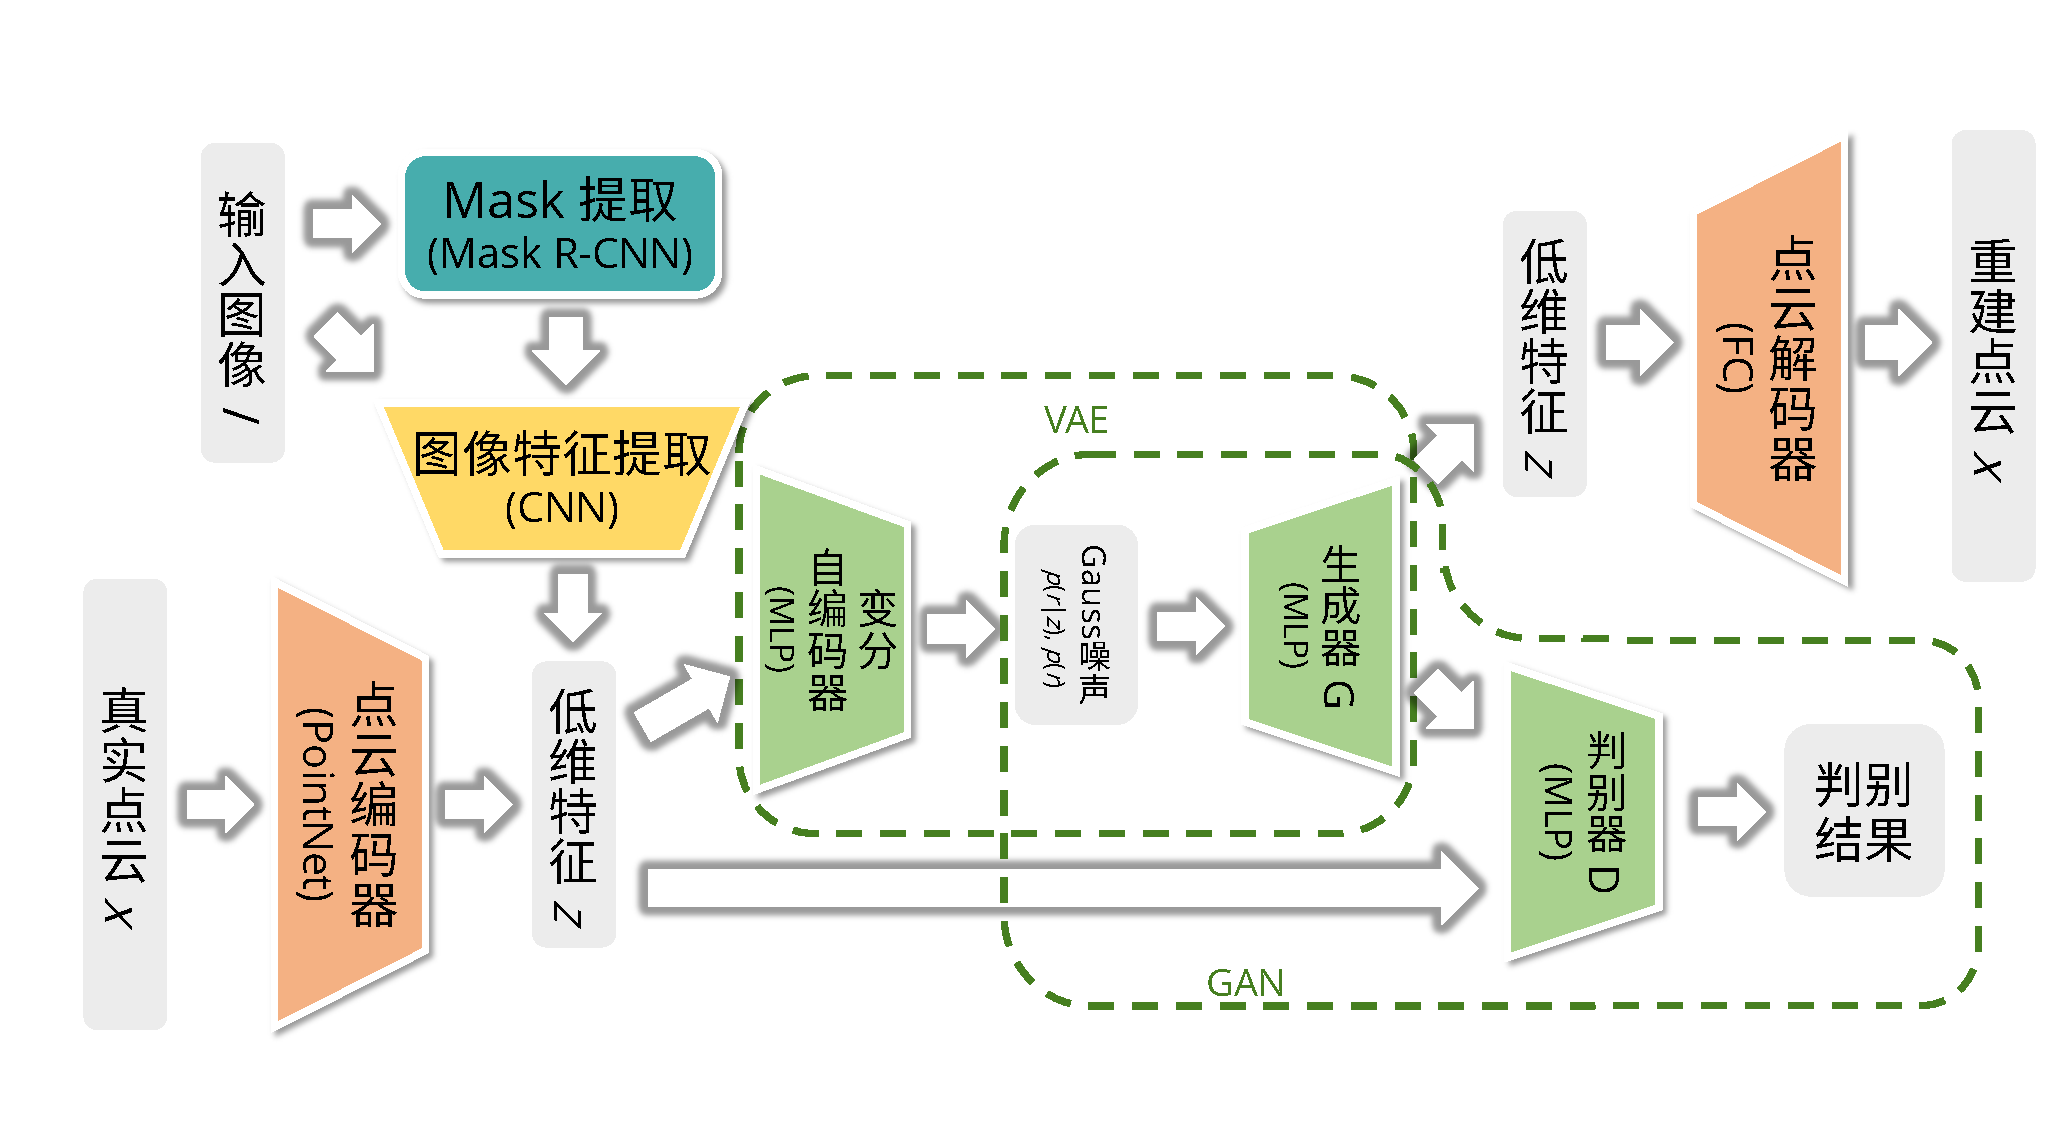
\includegraphics[width=.999\textwidth]{mystructure}}
	\caption{本工作的网络架构}
	\label{fig:mystructure}
\end{figure}

综上所述,为了解决第 \ref{section:myquestion} 节中提出的问题,我们使用如图 \ref{fig:mystructure} 所示
的%流水线
网络架构来处理用户的输入请求,%。%其中,
% 我们将各模块选取的网络架构标注在了右方。
其中,各模块所选取的具体%网络
架构被标注在了左方或下方位置。

% 要处理好做好流水线,
我们的%训练阶段
网络架构
% 主要
% 包括
%四个步骤
% 四部分
可以被粗略地分为四大组成部分
:点云自编码器(图 \ref{fig:mystructure} 橙红色部分)、Mask 生成模块(图 \ref{fig:mystructure} 青色部分)、图像特征提取模块(图 \ref{fig:mystructure} 黄色部分)以及 VAE/GAN(图 \ref{fig:mystructure} 绿色部分)。
我们将简要介绍这四部分的作用、目标及其%阶段%训练阶段%需要完成的任务
%的
训练方法。关于选取的模型架构与超参数的具体细节,请参见附录 \ref{cha:detail}。

\section{训练方法}
从图 \ref{fig:mystructure} 中可以看到,本工作的网络结构非常复杂。
事实上,本工作的训练过程也不是一步到位的,否则训练的代价太高;相反的,我们的训练过程按照模块的划分被分为四步。
本节介绍各模块的训练方法。
\subsection{点云自编码器\label{section:myae}}
点云自编码器 $E_{\text{AE}}, D_{\text{AE}}$ 对应图 \ref{fig:mystructure} 的橙红色部分。
它的核心目标是为了得到点云 $S = \bm x$ 的低维特征表示 $\bm z = E_{\text{AE}}(\bm x)$%。这样做的
。% 低维特征 $\bm z$ 
点云的低维特征 $\bm z$ 是后续训练流程所处理的基本对象。
%在后续训练的步骤中使用低维特征 $\bm z$ 的
相对于直接使用原始点云数据 $S = \bm x$,使用低维特征 $\bm z$ 有以下几点优势:
\begin{itemize}
	\item 能有效避免 PointNet\cite{pointnet} 鲁棒性带来的问题,%如同
	      正如
	      我们在第 \ref{section:rgan} 节中%所
	      提到的;%介绍的;
	\item 能有效加速后续步骤的运行速度,因为特征 $\bm z$ 的维数远远小于 $\bm x$ 的维数,后续步骤需要处理的数据规模大大降低;
	\item
	      % 提供了一个统一的标准,让图像提取模块可以和 VAE/GAN 结构自由对接。
	      能有效降低网络的复杂程度,减轻网络的负担:
	      例如,我们不必要求图像特征提取模块直接输出重建结果 $S = \bm x$,相反地,我们只要求它
	      % 只用
	      能够输出重建结果对应低维特征 $\bm z$ 即可。
	      重建出原始点云数据 $S$ 的任务将由解码器 $D_{\text{AE}}$ 进行进一步处理。
	      %否则,%若 GAN 的基本处理对象是点云,则

\end{itemize}

这个步骤只是一个预训练步骤,它的训练方法与第  \ref{section:gen3d} 节中 \inlinecite{latentpc} 工作提出的 l-GAN 如出一辙,此处不再赘述。
一旦预训练的过程完成,
%此训练步骤
%此步,
我们就固定编码器网络 $E_{\text{AE}}$ 和解码器网络 $D_{\text{AE}}$,并将特征
$\bm z = E_{\text{AE}}(\bm x)$ 视为数据集中的数据,不再考虑点云的原始表示 $\bm x$。

\subsection{Mask 生成模块 \label{my:mask}}
Mask 生成模块 $M$ 对应图 \ref{fig:mystructure} 的青色部分。
%此模块需要
其目的是
对用户提供的输入图像 $\bm I$ %上
进行物体分割,以自动生成出物体的 mask,使得后续的重建工作能够继续进行。

我们选择了 Mask R-CNN \cite{maskrcnn} 作为 mask 生成模块的网络架构。Mask R-CNN 是一个优秀的物体识别和语义分割算法,是早期工作 R-CNN\cite{rcnn}、Fast R-CNN\cite{fastrcnn}
、Faster R-CNN\cite{fasterrcnn} 的升级版本。相对于 Faster R-CNN,Mask R-CNN 增加了一个全卷积网络 (Fully Convolutional Network, FCN)分支,使得其能够胜任物体的分割任务。
由于物体检测和物体分割算法的具体实现并不是本文的讨论重点,因此我们不再单列章节%详细
展开介绍它们的具体细节和训练方法。%了。

在后期实验中,我们发现预训练好的 Mask R-CNN 对于小物体的分割非常准确,而对于大物体的分割就稍有欠缺了。%表现%就不那么好了。
究其原因,我们认为是其训练数据集%——
Microsoft Common Objects in Context (COCO) \cite{coco} 中小物体的数量远远多于大物体的数量%而
导致的。
而在本工作要解决的问题中,用户希望重建的物体是输入图像的主体,
其往往占据了整幅图像的绝大部分面积。这对于本工作而言是非常不利的。
% 往往会提供一张占据满整幅图像的

幸运的是,我们可以借助迁移学习的方法,提升 Mask R-CNN  在本问题上的表现。
具体而言,我们可以对于每一类物体,收集约 100 张占图像面积比例较高的大物体照片,
并手工标注其真实的 mask。利用这些新数据,我们在预训练好的 Mask R-CNN 进一步%继续
训练,直到 Mask R-CNN 能够比较好地完成大物体的分割任务为止。

\subsection{图像特征提取模块}
图像特征提取模块 $E_{\text{Image}}$ 对应图 \ref{fig:mystructure} 的绿色部分。
它的核心目标是:根据输入的 RGB 图像 $\bm I$ 和 mask $M(\bm I)$,计算图中三维模型点云表示 %$\bm x$ 
的低维特征 $\bm z = E_{\text{Image}}(\bm I_k, M(\bm I_k); \theta_{\text{Image}})$,以实现和 VAE/GAN\cite{vaegan} 以及解码器 $D_{\text{AE}}$ 的对接。
% 后面我们将会看到,
% 我们马上就可以
我们将会看到:
一旦特征 $\bm z$ 被计算出来,我们就可以使用 VAE/GAN 对其降噪,从而计算出一个更好的特征 $\bm z^*$,正如我们在第 \ref{section:vaegan} 节中所介绍的一样。
%此特征
经过%点云自编码器的
解码器 $D_{\text{AE}}$ 对此特征的进一步映射后,%后,%我们就可以得到
我们就得到了质量较好的重建结果 $S^* = \bm x^* = D_{\text{AE}}(\bm z^*)$。
这个点云降噪过程实现了%第 \ref{section:myquestion} 节中
提升重建模型质量 的基本要求。
% 这实现了 在第 \ref{section:myquestion} 节中 提出的提升重建模型质量 的基本要求。

% 正如在第 \ref{section:myae} 节中我们所强调的,图像特征提取模块不会涉及到任何点云原始数据 $\bm x$ 的计算,所有点云数据都是以其低维特征 $\bm z$ 的形式表现的。

在本工作中,图像特征提取模块的核心架构是卷积神经网络。这样的设计与 PointSetGen 是一脉相承的。由于卷积神经网络并不是本文介绍的重点,故其
具体细节此处不再赘述。

在训练时,我们希望最小化与模块输出与实际点云低维特征 $\bm z_{\text{gt}} = E_{\text{AE}}(\bm x_{\text{gt}})$ 之间的距离。即,对于数据集中的所有的图像 $\bm I$ 及其标注的真实点云 $\bm x_{\text{gt}} = S_{\text{gt}}$,我们希望最小化
\begin{align}
	\Loss(\bm \theta_{\text{Image}}) = \sum_k
	\Norm*{E_{\text{Image}}(\bm I_k, M(\bm I_k); \theta_{\text{Image}}) -
		E_{\text{AE}}(\bm x_{\text{gt}, k})}^2
	\label{eq:myimloss}
\end{align}
其中 $k$ 表示数据编号。

\subsection{VAE/GAN}
VAE/GAN 对应图 \ref{fig:mystructure} 的黄色部分,
包括了变分自编码器 $q(\bm r | \bm z; \bm\phi)$、
判别器 $D_{\text{GAN}}(\bm z)$、
生成器 $G_{\text{GAN}}(\bm r)$ 三部分。

通过第 \ref{section:gan} 、 \ref{section:vaegan} 节 的介绍,我们了解了 VAE/GAN\cite{vaegan}可以对图像进行插值和降噪。因此,我们把 VAE/GAN 引入到这个重建问题中,
并希望它能够实现增强重建质量与提升用户可控性这两点需求。%,如图\ref{section:myquestion}。

此处 VAE/GAN 的损失函数和训练方法与我们在第 \ref{section:vaegan} 节中介绍的 VAE/GAN 是基本类似的。
由于此处生成器 $G_{\text{GAN}}$ 从隐向量 $\bm r \sim \NormDist(\bm0, \bm I)$ 直接生成特征 $\bm z$,因此我们可以仿照 式 \eqref{eq:vaeganloss} 定义损失函数:
\begin{subequations}
	\label{eq:myvaeganloss}
	\begin{align}
		\Loss_{\text{KL}}          & = \DKL{q(\bm r | \bm z; \bm\phi)}{p(\bm r)}
		\\
		\Loss_{\text{reconstruct}} & = \EXPECT{\bm r\sim q(\bm r | \bm z; \bm \phi)}{\left[\Norm*{\bm z - G_{\text{GAN}}(\bm r)}^2\right]}
		\\
		\Loss_D                    & =
		- \EXPECT{\bm z \sim \PDATA(\bm z)}           \log(    D_{\text{GAN}}(\bm z))
		- \EXPECT{\bm r \sim \NormDist(\bm 0, \bm I)} \log(1 - D_{\text{GAN}}( G_{\text{GAN}}(\bm r)))
		\\
		\Loss_G                    & =
		- \EXPECT{\bm r \sim \NormDist(\bm 0, \bm I)} \log(D_{\text{GAN}}( G_{\text{GAN}}(\bm r)))
	\end{align}
\end{subequations}
而训练方法没有任何变化,仍然是交替优化:
\begin{subequations}
	\begin{align}
		\bm\theta_D^*    & = \argmin{\bm\theta_D} = \lambda_D \cdot \Loss_D \tag*{\ref{eq:vaegantrain1}}
		\\
		\bm\theta_\phi^* & = \argmin{\bm\theta_\phi} =
		\lambda_{\text{KL}} \cdot \Loss_{\text{KL}} +
		\lambda_{\text{reconstruct}} \cdot \Loss_{\text{reconstruct}} \tag*{\ref{eq:vaegantrain2}}
		\\
		\bm\theta_G^*    & = \argmin{\bm\theta_G} =
		\lambda_G \cdot \Loss_G +
		\lambda_{\text{reconstruct}} \cdot \Loss_{\text{reconstruct}} \tag*{\ref{eq:vaegantrain3}}
	\end{align}
\end{subequations}
其中 $\lambda_{\text{KL}}, \lambda_{\text{reconstruct}}, \lambda_D, \lambda_G$ 为平衡因子。

在第 \ref{section:gan}、\ref{section:ganimprove} 节中,我们介绍了经典 GAN 存在不稳定、训练困难的问题。
为了避免这种情况的发生,这里我们使用了谱标准化生成对抗网络 (Spectral Normalization Generative Adversarial Network, SNGAN)
\cite{sngan}。SNGAN 通过
限制判定器网络中每一层的谱半径
%单位化
为 $1$,有效地确保了 $D_{\text{GAN}}$ 满足 Lipschitz 连续条件 \eqref{eq:lip},增强了 GAN 训练过程的稳定性,且其速度优于其他试图改进 GAN 的工作。
限于篇幅,此处不再进一步展开介绍 SNGAN 及其相关工作。

% $\Norm{D_{\text{GAN}}}_{\text{Lip}} \le 1$,
% 其结构正是我们在

